\documentclass[aspectratio=169]{beamer}

\usetheme{Boadilla}
\usecolortheme{beaver}
\setbeamertemplate{navigation symbols}{}
\setbeamertemplate{footline}[frame number]

\usepackage[utf8]{inputenc}
\usepackage[brazil]{babel}
\usepackage{booktabs}
\usepackage{graphicx}
\usepackage{amsmath}
\usepackage{amssymb}
\usepackage{multirow}
\usepackage{xcolor}

% Figuras geradas pelos experimentos (rodada 1 — 1.476 chips)
\graphicspath{{../resultados/evaluation/}}

\definecolor{gain}{RGB}{0,128,0}
\definecolor{loss}{RGB}{180,0,0}

\title[FFL + SATLAS: Gap Espectral Planet--Aerofoto]{Superresolução no Domínio de Frequências\\\textit{Fine-tuning} do SATLAS com Focal Frequency Loss\\para Correção do Gap Espectral Planet--Aerofoto}
\author{Marcel Fernandes Gomes}
\institute{PPGC -- UFRGS \\ CMP570 -- Fotografia Computacional \\ Prof.\ Manuel M.\ de Oliveira Neto \\ Orientador: Prof.\ Dr.\ Eduardo S.\ L.\ Gastal}
\date{Junho de 2026}

% ============================================================
\begin{document}
% ============================================================

\begin{frame}
  \titlepage
\end{frame}

% ----------------------------------------------------------
\begin{frame}{Motivação: o \textit{gap} espectral Planet $\to$ aerofoto}

  \begin{columns}[T]
    \begin{column}{0.56\textwidth}
      \begin{itemize}
        \item Satélites comerciais de média resolução (PlanetScope,
              $\approx$3\,m/px) carecem de \textbf{detalhe fino} frente a aerofotos
              ($\approx$0{,}3--0{,}5\,m/px).
        \item Esse \textit{gap} aparece como \textbf{déficit de energia nas
              altas frequências} do espectro de potência (PSD).
        \item Limita aplicações que dependem de textura fina: infraestrutura
              urbana, cobertura vegetal, detecção de mudanças.
      \end{itemize}
      \begin{block}{Ideia central}
        Usar \textbf{superresolução por rede neural} para atenuar o \textit{gap}
        --- e medir o ganho \emph{no domínio de frequências}.
      \end{block}
    \end{column}
    \begin{column}{0.42\textwidth}
      \centering
      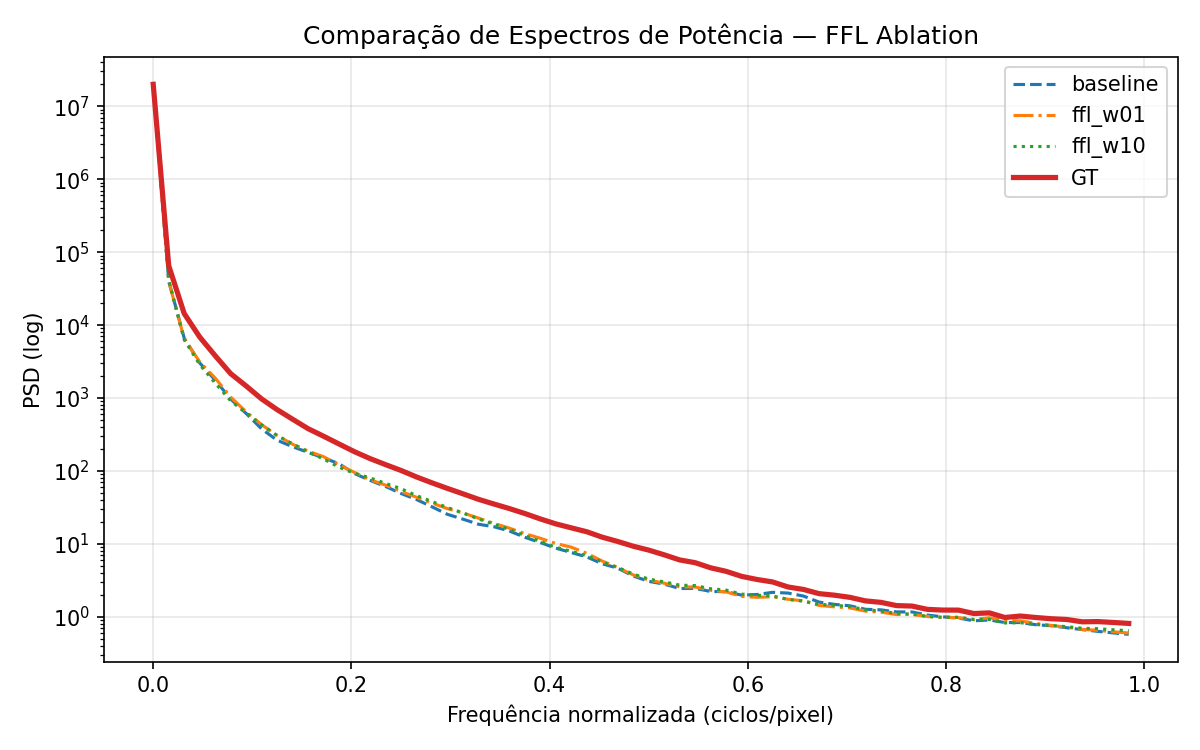
\includegraphics[width=\linewidth]{psd_comparison.png}\\
      {\small PSD radial: todas as variantes ficam \emph{abaixo} do GT
      nas frequências médias--altas.}
    \end{column}
  \end{columns}

\end{frame}

% ----------------------------------------------------------
\begin{frame}{Pergunta e contribuição}

  \begin{block}{Pergunta}
    A \textbf{Focal Frequency Loss} (FFL) consegue empurrar um gerador ESRGAN
    a recuperar as frequências altas que o L1 e a \textit{perceptual loss}
    tendem a suavizar?
  \end{block}

  \vspace{0.4em}
  \textbf{Abordagem:} \textit{fine-tuning} do \textbf{SATLAS} (ESRGAN pré-treinado
  Sentinel-2 $\to$ NAIP, $4\times$) com pares locais \textbf{Planet $\to$ aerofoto},
  adicionando a FFL como \textit{loss} auxiliar espectral.

  \vspace{0.6em}
  \begin{block}{\textit{Ablation study} --- 3 variantes}
    \begin{itemize}
      \item \textbf{Baseline}: L1 + Perceptual + GAN (sem FFL)
      \item \textbf{FFL $\lambda=0{,}1$}: FFL com peso baixo
      \item \textbf{FFL $\lambda=1{,}0$}: FFL com peso alto
    \end{itemize}
  \end{block}

  Avaliadas por \textbf{SSIM} (estrutura), \textbf{cPSNR} (reconstrução tolerante a
  \textit{offset} inter-sensor) e \textbf{PSD\_L2} (distância espectral ao GT).

\end{frame}

% ----------------------------------------------------------
\begin{frame}{Fundamentação: do gap à Focal Frequency Loss}

  \begin{columns}[T]
    \begin{column}{0.5\textwidth}
      \textbf{Caracterização do gap (Fourier 2D):}
      \[
        F[u,v] = \!\!\sum_{x,y}\! I[x,y]\,e^{-j2\pi\left(\frac{ux}{H}+\frac{vy}{W}\right)}
      \]
      PSD radial média $P(r)=|F|^2$ integrada em anéis $r=\sqrt{u^2+v^2}$.
      O \textit{gap} = queda mais acentuada da PSD do Planet vs.\ aerofoto.

      \vspace{0.5em}
      \begin{block}{\textit{Loss} total}
        \[
          \mathcal{L} = \mathcal{L}_{L1} + \lambda_{p}\mathcal{L}_{p}
          + \lambda_{G}\mathcal{L}_{G} + \textcolor{loss}{\lambda_{FFL}\mathcal{L}_{FFL}}
        \]
      \end{block}
    \end{column}
    \begin{column}{0.5\textwidth}
      \textbf{Focal Frequency Loss} (Jiang et al., ICCV 2021):
      \[
        \mathcal{L}_{FFL} = \frac{1}{MN}\sum_{u,v} w[u,v]\,
        \big|F_{\hat{I}}[u,v]-F_{HR}[u,v]\big|^2
      \]
      \begin{itemize}
        \item $w[u,v]$ = máscara \textbf{adaptativa}, atualizada a cada iteração.
        \item Frequências bem recuperadas: $w\!\approx\!0$.
        \item Mal recuperadas (altas): $w\!\approx\!1$ $\Rightarrow$ recebem
              \textbf{mais gradiente}.
      \end{itemize}
      \vspace{0.3em}
      \textcolor{gain}{Reequilibra o gradiente que o L1 (dominado por baixas
      frequências) enviesa.}
    \end{column}
  \end{columns}

\end{frame}

% ----------------------------------------------------------
\begin{frame}{Conexão com os tópicos de CMP570}

  \begin{center}
  \begin{tabular}{ll}
    \toprule
    \textbf{Tópico (CMP570)} & \textbf{Papel no projeto} \\
    \midrule
    Aulas 12--13 — Fourier / DFT      & \texttt{torch.fft.fft2} no núcleo da FFL \\
    Aula 14 — Aliasing / Nyquist      & Motivação do gap espectral Planet/Sentinel \\
    Aula 15 — Teorema da Convolução   & Relação PSF $\leftrightarrow$ domínio de frequência \\
    Semanas 10--11 — Filtro de Wiener & \textit{Baseline} clássico de comparação \\
    \bottomrule
  \end{tabular}
  \end{center}

  \vspace{1em}
  \begin{block}{Síntese}
    O trabalho leva os tópicos do curso a um problema real de sensoriamento
    remoto: \textbf{usar o domínio de frequências tanto como ferramenta de
    treino (FFL) quanto como métrica de avaliação (PSD\_L2)}.
  \end{block}

\end{frame}

% ----------------------------------------------------------
\begin{frame}{Metodologia --- dados, implementação e treino}

  \begin{columns}[T]
    \begin{column}{0.5\textwidth}
      \textbf{Dados}
      \begin{itemize}\small
        \item Entrada: PlanetScope (4 bandas, 3\,m/px), RS.
        \item GT: aerofoto $\approx$0{,}5\,m/px, mesma região.
        \item Chips $32\!\times\!32$ (LR) $\to$ $128\!\times\!128$ (HR),
              escala $4\times$, alinhados via GDAL/rasterio.
      \end{itemize}

      \vspace{0.3em}
      \textbf{FFL no SATLAS} (2 patches, retrocompatíveis)
      \begin{itemize}\small
        \item \texttt{losses/basic\_loss.py}: classe
              \texttt{FocalFrequencyLoss} no \texttt{LOSS\_REGISTRY}.
        \item \texttt{models/ssr\_esrgan\_model.py}: campo
              opcional \texttt{ffl\_opt} no YAML.
      \end{itemize}
    \end{column}
    \begin{column}{0.5\textwidth}
      \fontsize{8.5pt}{11pt}\selectfont
      \begin{tabular}{ll}
        \toprule
        \textbf{Parâmetro} & \textbf{Valor} \\
        \midrule
        Ponto de partida   & \texttt{esrgan\_16S2.pth} \\
        Iterações          & 20.000 \\
        Batch size         & 4 \\
        LR inicial         & $10^{-4}$ (decai 8k/16k) \\
        $N_s$ imagens/amostra & 16 \\
        Chips treino/val   & 1.476 \\
        $\lambda_{L1}/\lambda_{p}/\lambda_{G}$ & 1{,}0 / 1{,}0 / 0{,}1 \\
        $\lambda_{FFL}$    & 0 / 0{,}1 / 1{,}0 \\
        \bottomrule
      \end{tabular}

      \vspace{0.5em}
      {\small GPU Tesla V100-32GB, CUDA 12.9. Mesmo orçamento de treino
      (iter 20k fixo) para comparação justa.}
    \end{column}
  \end{columns}

\end{frame}

% ----------------------------------------------------------
\begin{frame}{Resultado principal --- FFL $\lambda=1{,}0$ recupera frequências}

  \begin{columns}[T]
    \begin{column}{0.46\textwidth}
      \fontsize{9pt}{12pt}\selectfont
      \begin{tabular}{lccc}
        \toprule
        \textbf{Variante} & \textbf{SSIM}$\uparrow$ & \textbf{cPSNR}$\uparrow$ & \textbf{PSD\_L2}$\downarrow$ \\
        \midrule
        Baseline             & 0,6352 & 29,09 & 0,2574 \\
        FFL $\lambda{=}0{,}1$ & \textbf{0,6368} & 29,08 & 0,2638 \\
        \textcolor{gain}{FFL $\lambda{=}1{,}0$} & 0,6291 & 29,03 & \textcolor{gain}{\textbf{0,2389}} \\
        \bottomrule
      \end{tabular}

      {\fontsize{7.5pt}{9pt}\selectfont iter 20.000 --- 1.476 chips.}
      \vspace{0.5em}
      \begin{itemize}\small
        \item \textcolor{gain}{\textbf{PSD\_L2 $-$7,2\%}} vs.\ baseline ---
              a FFL fecha parte do gap espectral.
        \item Custo \textbf{pequeno}: $\Delta$SSIM $=-0{,}006$;
              $\Delta$cPSNR $=-0{,}06$\,dB.
        \item \textit{Trade-off} favorável p/ fidelidade espectral.
      \end{itemize}
    \end{column}
    \begin{column}{0.52\textwidth}
      \centering
      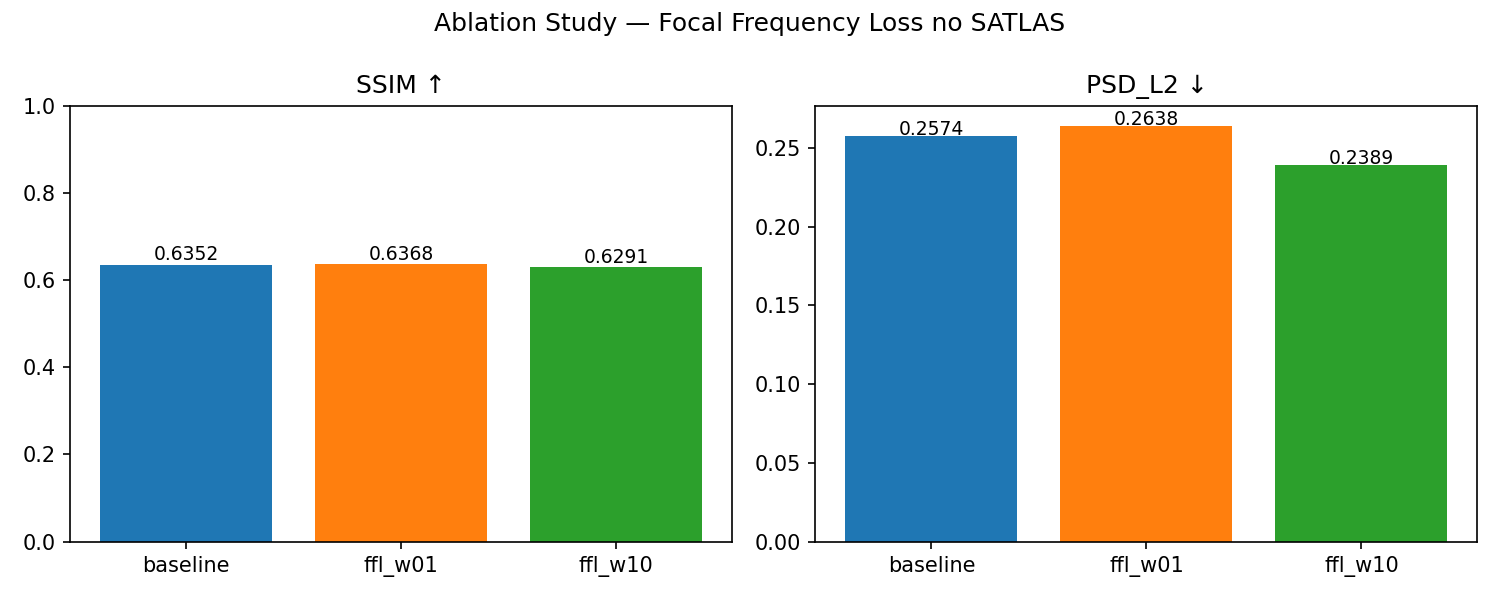
\includegraphics[width=\linewidth]{metrics_comparison.png}\\
      {\small SSIM (esq.) e PSD\_L2 (dir.): $\lambda=1{,}0$ tem o melhor
      equilíbrio espectral.}
    \end{column}
  \end{columns}

\end{frame}

% ----------------------------------------------------------
\begin{frame}{Discussão --- por que funciona (e por que $\lambda=0{,}1$ não)}

  \begin{block}{Mecanismo}
    O L1 minimiza erro pixel a pixel, dominado pelas \textbf{baixas frequências}
    (maior energia $\Rightarrow$ maior contribuição ao MSE). Resultado: estrutura
    grossa boa, \textbf{texturas finas suavizadas}. A FFL pondera o erro espectral
    de forma adaptativa e \textbf{redireciona o gradiente às frequências altas}.
  \end{block}

  \vspace{0.4em}
  \begin{itemize}
    \item \textbf{$\lambda=1{,}0$:} o gerador ``sacrifica'' alinhamento estrutural
          (queda de SSIM) para ganhar energia em alta frequência (queda de PSD\_L2)
          --- o \textit{trade-off} típico espectral vs.\ espacial.
    \item \textbf{$\lambda=0{,}1$ insuficiente:} o gap Planet$\to$aerofoto é grande
          demais; o peso baixo não ativa o mecanismo focal.
    \item \textbf{Métrica espectral importa:} SSIM/PSNR não capturam o ganho ---
          só o PSD\_L2 revela o efeito que a FFL visa corrigir.
  \end{itemize}

\end{frame}

% ----------------------------------------------------------
\begin{frame}{Conclusão e trabalhos futuros}

  \begin{block}{Resposta à pergunta central}
    \textbf{Sim:} a FFL com $\lambda=1{,}0$ reduz o PSD\_L2 em \textbf{7,2\%} frente
    ao baseline, com custo de SSIM desprezível --- confirmando que a \textit{loss}
    espectral recupera frequências altas suavizadas pelas \textit{losses}
    convencionais.
  \end{block}

  \vspace{0.3em}
  \textbf{Contribuições:}
  \begin{enumerate}
    \item Integração retrocompatível da FFL ao SATLAS/BasicSR.
    \item \textit{Ablation} controlado (mesmo orçamento de treino) no domínio
          Planet$\to$aerofoto.
    \item Avaliação espectral (PSD\_L2) que expõe ganhos invisíveis a SSIM/PSNR.
  \end{enumerate}

  \vspace{0.3em}
  \textbf{Trabalhos futuros:} pesos intermediários ($\lambda=0{,}3$, $0{,}5$);
  mais dados / maior área (rodada 2 --- $\sim$9{,}4k chips em andamento);
  comparação com outros métodos guiados por frequência.

\end{frame}

% ----------------------------------------------------------
\begin{frame}[plain]
  \begin{block}{Mensagem central}
    O domínio de frequências é, ao mesmo tempo, \textbf{a ferramenta} (FFL guiando o
    treino) e \textbf{a métrica} (PSD\_L2 medindo o gap). Ponderar o erro espectral
    de forma adaptativa basta para que um gerador ESRGAN recupere frequências altas
    que as \textit{losses} espaciais deixam escapar.
  \end{block}
  \vspace{3em}
  \begin{center}
    \Large\textbf{Obrigado!}\\[0.6em]
    \normalsize marcelgfernandes@gmail.com
  \end{center}
\end{frame}

% ============================================================
\end{document}
